\pdfoutput=1
\pdfcompresslevel=9
\pdfinfo
{
    /Author ()
    /Title ()
    /Subject ()
    /Keywords ()
}
\documentclass[a4paper,onecolumn,oneside,12pt]{mwrep}

\usepackage{times}
\usepackage[utf8x]{inputenc}
\usepackage[T1]{fontenc}
\usepackage[polish]{babel}
\usepackage{setspace}
\usepackage{graphicx} 

\hyphenpenalty=10000		% nie dziel wyrazów zbyt często
\clubpenalty=10000			% kara za sierotki
\widowpenalty=10000			% nie pozostawiaj wdów
\brokenpenalty=10000		% nie dziel wyrazów między stronami
\exhyphenpenalty=999999		% nie dziel słów z myślnikiem
\righthyphenmin=3			% dziel minimum 3 litery

\tolerance=4500
\pretolerance=250
\hfuzz=1.5pt
\hbadness=1450

\sloppy						% umacnia pozycję prawego marginesu

\setlength{\textwidth}{\paperwidth}
\addtolength{\textwidth}{-5cm}
\setlength{\textheight}{\paperheight}
\addtolength{\textheight}{-5cm}
\setlength{\oddsidemargin}{0cm}
\setlength{\evensidemargin}{0cm}
\topmargin -1.25cm
\footskip 1.4cm

\linespread{1.3}

\begin{document}

\begin{titlepage}
	\begin{center}
	    \fontsize{14pt}{12px}\selectfont
        \textbf{POLITECHNIKA WARSZAWSKA} \\
        WYDZIAŁ ELEKTRYCZNY \\
        INSTYTUT STEROWANIA I ELEKTRONIKI PRZEMYSŁOWEJ
        
	    \vspace*{.6\baselineskip}
	    
	    \fontseries{b}\fontsize{12pt}{10pt}\selectfont
	    PRACA DYPLOMOWA MAGISTERSKA \\
        na kierunku INFORMATYKA \\
        specjalność: inżynieria oprogramowania
	\end{center}
	
	\begin{flushleft}
        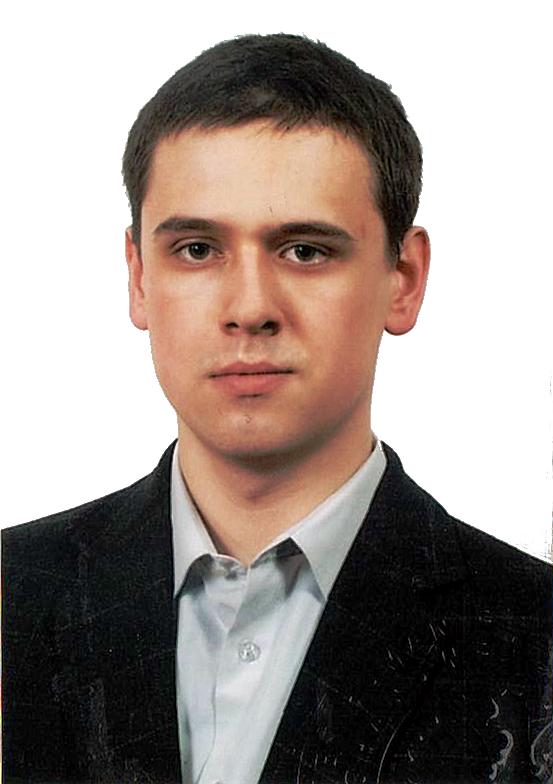
\includegraphics[width=4cm]{img/zdjecie_dyplo.png} \\
	    \fontsize{14pt}{12px}\selectfont
        Jakub SAŁKOWSKI \\
	    \fontseries{b}\fontsize{12pt}{10pt}\selectfont
        Nr albumu: 248418
    \end{flushleft}
	
	\begin{flushright}
    	\begin{minipage}{0.3\textwidth}
    	    \fontsize{12pt}{10pt}\selectfont
    	    Rok akad.: 20013/2014 \\		
    	    \fontsize{10pt}{8pt}\selectfont
            Warszawa, \textit{2013.05.12}
        \end{minipage}
	\end{flushright}
	
	\vspace*{1\baselineskip}
	    
	\begin{center}
	    \fontseries{b}\fontsize{14pt}{12pt}\selectfont
	    PROJEKT APLIKACJI ODCZYTUJĄCEJ NUMER 
	    NADJEŻDŻAJĄCEGO AUTOBUSU NA URZĄDZENIA
	    MOBILNE Z~SYSTEMEM ANDROID \\
	\end{center}
	
	\vspace*{1\baselineskip}
	
	\begin{flushleft}
	    \fontseries{b}\fontsize{12pt}{10pt}\selectfont
	    Zakres pracy:
	    \fontseries{m}\fontshape{it}\selectfont
	    \begin{enumerate}
	        \item Wprowadzenie i~sformułowanie celu pracy
	        \item Przegląd dostępnych technik detekcji
	        i~identyfikacji obiektów w obrazach
	        \item Przygotowanie środowiska usprawniającego
	        implementację i~weryfikację wybranych algorytmów
	        \item Analiza porównawcza najbardziej obiecujących
	        metod detekcji i~identyfikacji obiektów w~obrazach
	        \item Implementacja i~weryfikacja algorytmu
	        obdarzonego największym potencjałem na kilku
	        urządzeniach z~systemem Android
	        \item Wnioski i~podsumowanie
	    \end{enumerate}
	    \fontshape{n}\fontseries{b}
	    \fontsize{12pt}{10pt}\selectfont
	    
	    \vspace*{1\baselineskip}
	
	    Kierujący pracą: \textit{dr inż. Witold Czajewski} \\
	    
	    \vspace*{4\baselineskip}
	    
	    \fontseries{m}\selectfont
	    Termin złożenia pracy: \textit{2014.09.15} \\
	    \fontsize{10pt}{8pt}\selectfont
        Praca wykonana i obroniona pozostaje \\
        własnością Instytutu, Katedry i nie będzie \\
        zwrócona wykonawcy.
	\end{flushleft}
\end{titlepage}

% streszczenie
\begin{center}
\textbf{Streszczenie}
\end{center}

Lorem ipsum dolor sit amet, consectetuer adipiscing elit. Donec vitae ipsum ut
libero lacinia sodales. Nunc nec diam quis felis congue aliquet. Proin hendrerit
urna eget mauris.

\vspace*{\baselineskip}

\noindent\textbf{Słowa kluczowe:} \textit{asercja, optymalizacja.}

\vspace*{2\baselineskip}

\begin{center}
\textbf{Abstract}
\end{center}

Lorem ipsum dolor sit amet, consectetuer adipiscing elit. Donec vitae ipsum ut
libero lacinia sodales. Nunc nec diam quis felis congue aliquet. Proin hendrerit
urna eget mauris.

\vspace*{\baselineskip}

\noindent\textbf{Keywords:} \textit{asercja, optymalizacja.}

\setcounter{page}{2}

\tableofcontents

\chapter{Wprowadzenie}

Widzenie maszynowe jest jedną z~najprężniej rozwijających się
dziedzin z~pogranicza algorytmiki, optymalizacji, przetwarzania obrazów,
przetwarzania sygnałów, statystyki oraz szeroko pojętej sztucznej
inteligencji, jeżeli chodzi o~zagadnienia informatyczne w~ostatnich
latach. Sporządzenie definicji widzenia komputerowego jest niezmiernie
trudne. Głównie z~powodu wspomnianej interdyscyplinarności
jaką niesie ze sobą omawiany termin. Klasyczne, jednozdaniowe
definicje przedstawiają w~zwięzły sposób ogólny zarys koncepcji
jaka kryje się za sformułowaniami określanymi mianem wizji komputerowej.
Wysoki poziom abstrakcji oraz zwięzłość formy zmuszają do pominięcia
wielu istotnych aspektów, które nienaświetlone mogą w~poważny sposób
zaburzyć wyobrażenie o~tym niezmiernie interesującym 
obszarze nauki i~techniki.  
Poniżej przedstawiono kilka definicji wprowadzonych na przestrzeni
kilkunastu ostatnich lat. 

DEFINICJA 1 \cite{ShapiroStockman200102}:

,,Zadaniem wizji komputerowej jest podejmowanie 
decyzji na temat rzeczywistych (fizycznych) obiektów
oraz scen na podstawie obrazów.''

W~komentarzu do zaprezentowanej definicji wprowadzony został
cel pośredni. Aby podjęcie decyzji na temat rzeczywistych obiektów
było możliwe, niemal zawsze niezbędne jest sporządzenie ich modelu lub 
opisu na podstawie posiadanych zdjęć. Zgodnie z~powyższym,
równolegle do poprzedniej definicji, zaproponowana została druga, mniej
abstrakcyjną wersja, którą umieszczono poniżej.

DEFINICJA 2 \cite{ShapiroStockman200102}:

,,Zadaniem wizji komputerowej jest sporządzanie
opisów scen rzeczywistych na podstawie obrazów.''

Jest to pierwsza próba ograniczenia danych wyjściowych jakich należałoby
oczekiwać po uruchomieniu procesu określanego mianem wizji komputerowej.

Następna definicja jest kolejną próbą
podjętą w~kierunku maksymalnego uproszczenia i~zawężenia
przeciwdziedziny widzenia komputerowego. Nie ulega raczej wątpliwości,
że danymi wejściowymi procesu są obrazy lub sekwencje obrazów.
W~tym kontekście następne zdanie definiuje produkt omawianego zagadnienia.

DEFINICJA 3 (na podstawie \cite{morris2004computer}):

,,Wizja komputerowa obejmuje swym zakresem wydobywanie
danych numerycznych z~obrazów.''

Tak jak przetwarzanie obrazów określa działania na obrazach wynikiem
których są obrazy o~zmienionych właściwościach w~porównaniu do obrazów
wejściowych, tak wynikiem widzenia komputerowego są dane wydobywane
z~obrazów. Dane wyłuskane w~ten sposób mogą zostać wykorzystane
na wiele sposobów:
\begin{itemize}
    \item prezentując wartość samą w~sobie, np.: odczyt tekstu
        z~zeskanowanych dokumentów (OCR),
    \item określając współrzędne elementów sceny, w~kontekście OCR 
        i~odczytywania tekstu z~dokumentów dane tego typu
        wykorzystywane są do zachowania struktury dokumentu, tabel,
        obrazów itp.
    \item do uwierzytelniania na podstawie danych biometrycznych - 
        rozpoznawanie i~identyfikacja siatkówki oka,
    \item do budowania modeli trójwymiarowych obiektów na podstawie 
        sekwencji obrazów, itp.
\end{itemize}

Jak łatwo zauważyć widzenie komputerowe to niezwykle pojemny termin.
Interdyscyplinarność czyni próbę wymienienia zagadnień z~nim związanych,
bez pominięcia jakiejś istotnej gałęzi, niemal niemożliwą. 
Złożoność i~rozległość zakresu jaki wiąże się
z~tym zagadnieniem zilustrowano na rys. \ref{fig:int_cv_inter_discip}.

\begin{figure}[!h]
    \centering
    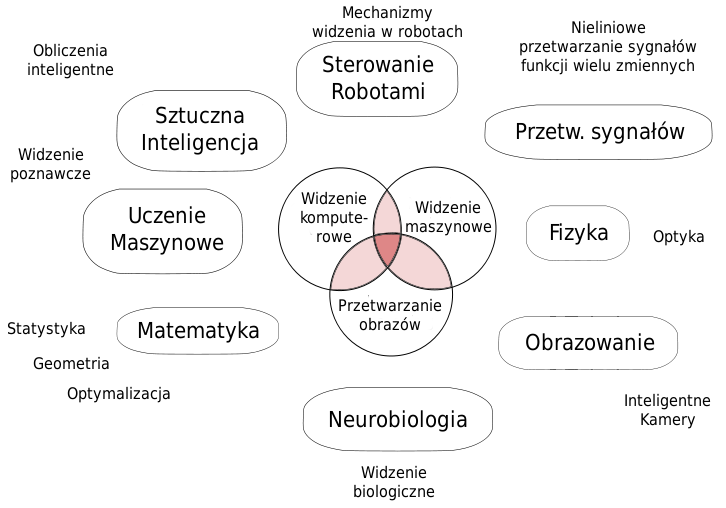
\includegraphics[width=0.9\textwidth]{img/int_cv_inter_discip}
    \caption{Powiązanie wizji komputerowej z~innymi dziedzinami 
        (na podstawie \cite{wiki:computervision})}
    \label{fig:int_cv_inter_discip}
\end{figure}

Narodziny widzenia maszynowego miały
miejsce na początku drugiej połowy ubiegłego wieku.
W~latach pięćdziesiątych wdrożone zostały dwie implementacje 
pierwszego komercyjnego systemu OCR (\textit{ang. Optical Character 
Recognition}). Pierwszym klientem było wydawnictwo Reader's Digest,
gdzie system wykorzystywano do automatycznego odczytywania adresów
z~przesyłek wysyłanych do czytelników w~celu ich sortowania.
Drugim klientem komercyjnego systemu OCR 
była firma Standard Oil Company. Rozwiązanie
służyło odczytywaniu danych z~kart kredytowych w~celach 
rozliczeniowych \cite{WEB:ocrhistory}.

Obecnie istnieje wiele narzędzi do odczytywania tekstu z~zeskanowanych
dokumentów. Najlepsze rozwiązanie dostępne na rynku
można nabyć za cenę zbliżoną do tej w~jakiej oferowany jest
popularny pakiet oprogramowania biurowego.

Według innego opracowania \cite{web:huangcvevolution}
początki widzenia komputerowego są związane z~nazwiskiem Larrego
Robertsa. On to przez swoją pracę doktorską na temat możliwości
wyłuskania trójwymiarowych współrzędnych brył geometrycznych
z~dwuwymiarowych widoków perspektywicznych został okrzyknięty
,,ojcem'' wizji komputerowej. Praca została złożona i~obroniona 
w~latach 60 na uczelni MIT \cite{books/garland/Roberts63}.

Ważnym wydarzeniem z~perspektywy niniejszej pracy dyplomowej była
pierwsza implementacja algorytmu wykrywającego wystąpienie twarzy
w~obrazie w~czasie rzeczywistym.
Na początku obecnego stulecia opracowano oraz zaimplementowano algorytm
\cite{DBLP:conf/cvpr/ViolaJ01}, który uruchomiony na komputerze 
z~procesorem Intel Pentium III 700 MHz był w~stanie przeszukiwać obrazy
pod kątem wystąpienia twarzy w~tempie 15 klatek na sekundę.
Rozdzielczość obrazów wejściowych była równa 384 na 288 pikseli.
Dzisiaj, ze względu na moc obliczeniową urządzeń mobilnych, algorytm ten 
bez trudu można uruchomić
na telefonie lub aparacie fotograficznym. 
Ponadto uzyskane wyniki przekraczają wspomniane 15  na sekundę
przy jednoczesnym wykorzystaniu obrazów wejściowych w~znacznie
większej rozdzielczości: 720p czy nawet 1080p.
Jedną z~bardziej 
popularnych funkcjonalności opartych na wspomnianym rozwiązaniu 
jest wykorzystywany od kilku lat system zwalniania migawki w~aparatach
cyfrowych.
Zdjęcie wykonywane jest
po wykryciu twarzy w~kadrze zawierającej określony grymas, na przykład
uśmiech.

Moc obliczeniowa współczesnych smartfonów pozwala na uruchomienie
znacznie bardziej skomplikowanych algorytmów. Najnowsze jednostki,
wyposażone w~procesory cztero- i~ośmiordzeniowe można nabyć
w~cenie już kilkuset złotych. Dodatkowo mnogość dostępnych bibliotek 
sprawia, że głównym ograniczeniem przy projektowaniu i~implementacji
rozwiązań z~dziedziny widzenia komputerowego jest już niemal
tylko wyobraźnia. Co prawda, utrudnieniem może być słabej jakości
kamera dostępna w~urządzeniu, jednak ograniczenie to obowiązuje
tylko podczas implementacji algorytmów precyzyjnej lokalizacji
i~rozpoznawania obiektów na podstawie danych z~aparatu.

Jednym z~popularniejszych zastosowań widzenia komputerowego w~telefonach
jest odczytywanie kodów QR. Jest to często stosowana technika
np. w~muzeach. Aplikacje udostępniane przez placówki 
umożliwiają uzyskanie szczegółowych opisów eksponatów na
podstawie zamieszczonych obok nich kodów. Zwiedzający mogą w~ten sposób 
skorzystać z~towarzystwa wirtualnego przewodnika. 

Osobną grupę aplikacji stanowią programy napisane z~myślą 
o~niewidomych. W~skład zbioru wchodzą między innymi aplikacje
do rozpoznawania banknotów, obiektów na podstawie
naklejonych kodów QR, odczytywania napisów itp.
Zasadnym wydaje się więc istnienie aplikacji odczytującej numer 
autobusu właśnie w~kontekście wykorzystania przez osoby niewidome lub
niedowidzące. 

Celem niniejszej pracy jest przygotowanie działającej implementacji
algorytmu odczytującego numer zawarty we froncie nadjeżdżającego
autobusu na urządzeniu mobilnym z~systemem Android.
Do osiągnięcia ostatecznego celu niezbędna jest
realizacja następujących celów pośrednich:

\begin{itemize}
    \item przygotowanie
oraz weryfikacja algorytmu detekcji frontów autobusów w~scenie,
    \item lokalizacja numeru linii we froncie autobusu,
    \item rozpoznanie poszczególnych cyfr zawartych
        w~zlokalizowanym fragmencie frontu - odczytanie numeru. 
\end{itemize}

\begin{figure}[!h]
    \centering
    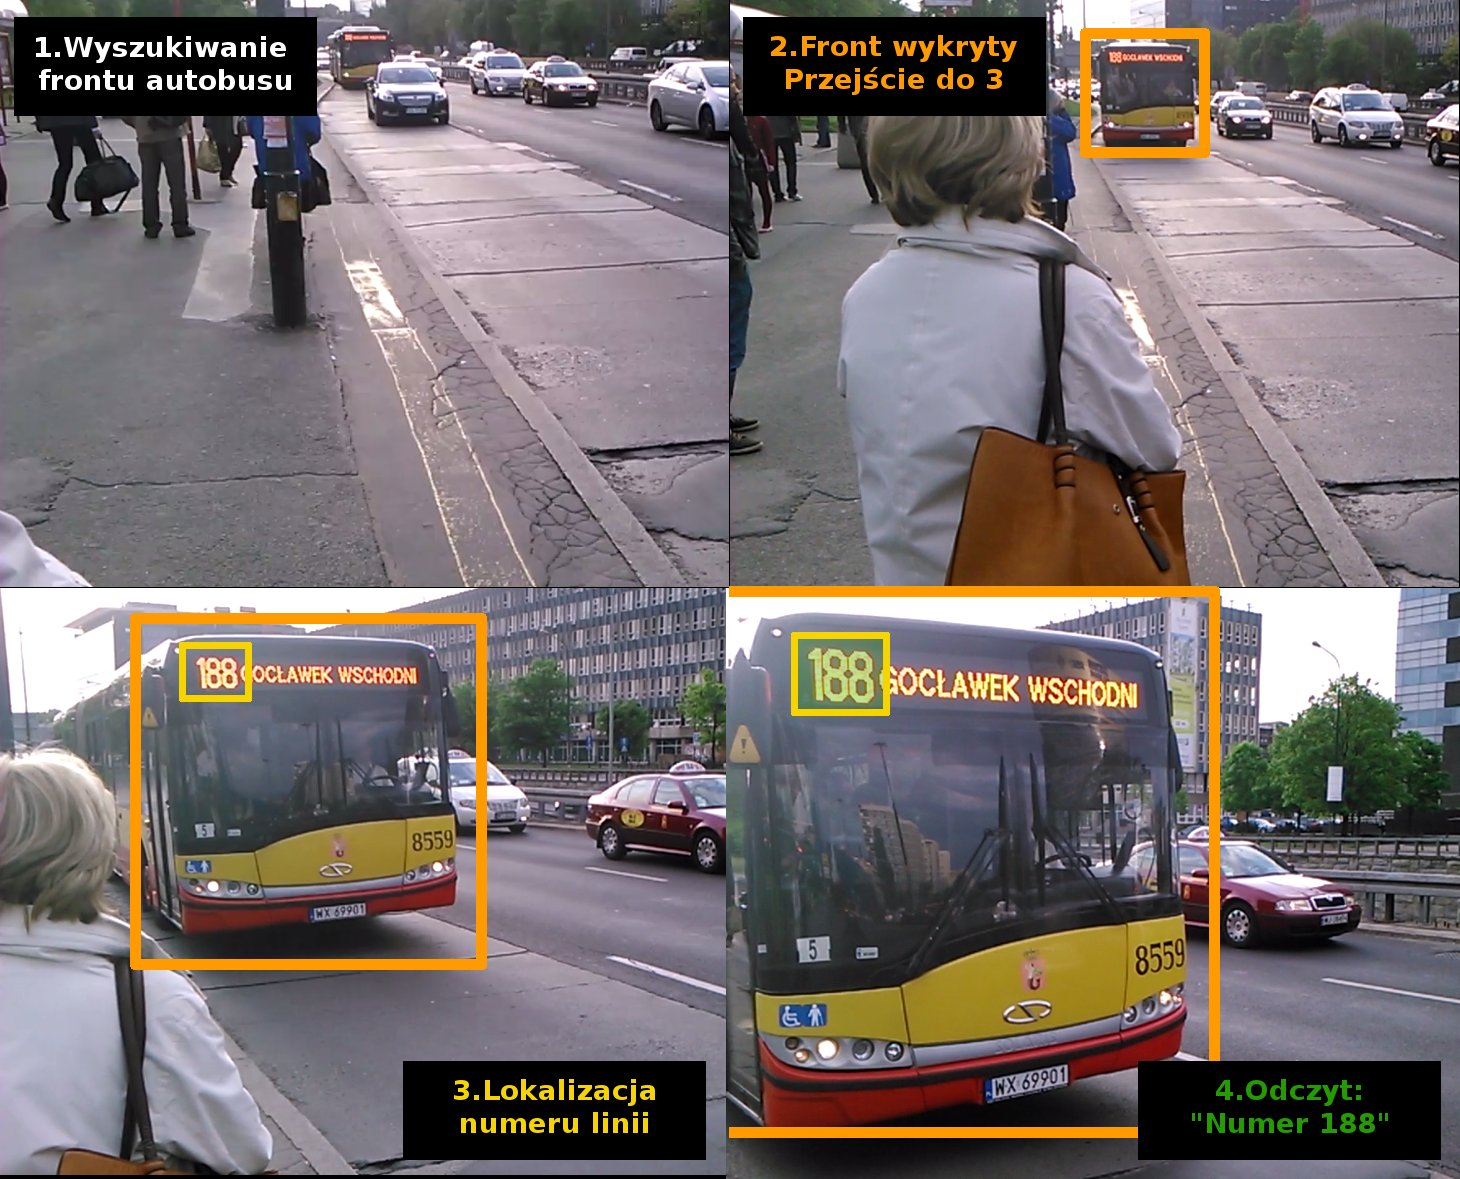
\includegraphics[width=0.9\textwidth]{img/int_use_case_sequence}
    \caption{Diagram przedstawiający przypadek użycia proponowanej aplikacji}
    \label{fig:int_use_case_diag}
\end{figure}

Elementem dodatkowym, nadającym sens całemu rozwiązaniu w~kontekście
wykorzystania aplikacji przez osoby niewidome i~niedowidzące,
byłoby wykorzystanie syntezatora tekstu na mowę dla 
odczytanego przez algorytm ciągu znaków reprezentującego numer linii. 
Scenariusz wykorzystania aplikacji zaprezentowano na rysunku
\ref{fig:int_use_case_diag}.


\section{Zakres pracy}

W~kolejnym rozdziale zawarto przegląd dostępnych implementacji związanych
z~detekcją i~identyfikacją obiektów. Wprowadzono obowiązujące
w~tej pracy definicje detekcji i~identyfikacji. 
Omówione zostały metody wykrywania obiektów, przy czym uwagę skupiono
głównie na istniejących rozwiązaniach, algorytmach, narzędziach 
i~bibliotekach. Ze względu na mnogość implementacji - dostępność 
na wielu platformach i~w~wielu językach - duży nacisk położono 
na bibliotekę OpenCV. Opisano zaskakująco dobre
rezultaty doświadczeń z~biblioteką OpenTLD, oraz problemy
na jakie natrafiono.

W~trzecim rozdziale przedstawiono proces implementacji
narzędzi wykorzystanych do zbudowania środowiska deweloperskiego
oraz testowego.

Kolejny - czwarty rozdział - zawarł opis i~podsumowanie wykonanych doświadczeń.
W~pierwszej kolejności zamieszczono opis 
prób testowych, przeprowadzonych w~celu identyfikacji najodpowiedniejszych 
narzędzi. Metody przedstawione 
w~tym rozdziale nie zostały wykorzystane w~rozwiązaniu końcowym.
Podsumowanie rozdziału czwartego to opis prób przeprowadzonych z~wykorzystaniem
kompletnej
implementacji, uruchamianej na komputerze stacjonarnym.

Ostatni - piąty rozdział - to zbiór wyników i~opisów doświadczeń 
wykonanych po implementacji rozwiązania na 
systemie docelowym. W~pierwszej kolejności
zbadano wydajność i~złożoność obliczeniową proponowanego rozwiązania.
Po zbadaniu czasów wykonania przeprowadzony został automatyczny test na 3000 obrazów
reprezentujących fronty autobusów. Ostatnim zagadnieniem były testy terenowe.
Opisano napotkane problemy środowiskowe i~ograniczenia technologiczne.

W~podsumowaniu jeszcze raz opisane zostały problemy i~ograniczenia.
Pokrótce wspomniano o~możliwościach rozwoju aplikacji i~możliwych usprawnieniach.
Ostatecznie przedstawiono rozwiązania alternatywne, ich wady i~zalety
w~porównaniu do systemu, który powstał w~ramach tej pracy.


\bibliography{sample}
\nocite{*}
\bibliographystyle{plain}

\end{document}

% ex: set tabstop=4 shiftwidth=4 softtabstop=4 noexpandtab fileformat=unix filetype=tex spelllang=pl,en spell:

